% quantum macros

\def\01{\{0,1\}}
\def\eps{\epsilon}
\newcommand{\half}{{\frac{1}{2}}}
\newcommand{\set}[1]{{\left\{#1\right\}}}
\newcommand{\ksubsets}{{n \choose k}}
\newcommand{\jsubsets}{{n \choose j}}
\newcommand{\Prob}{{\mathbf{Pr}}}
\newcommand{\tinyspace}{\mspace{1mu}}
\newcommand{\microspace}{\mspace{0.5mu}}
\newcommand{\op}[1]{\operatorname{#1}}

\newcommand{\norm}[1]{\left\lVert\tinyspace#1\tinyspace\right\rVert}
\newcommand{\snorm}[1]{\lVert\tinyspace#1\tinyspace\rVert}
\newcommand{\abs}[1]{\left\lvert\tinyspace #1 \tinyspace\right\rvert}
\newcommand{\ceil}[1]{\left\lceil #1 \right\rceil}
\newcommand{\floor}[1]{\left\lfloor #1 \right\rfloor}
\def\iso{\cong}
\newcommand{\defeq}{\stackrel{\smash{\text{\tiny def}}}{=}}
\newcommand{\tr}{\operatorname{tr}}
\newcommand{\rank}{\operatorname{rank}}
\renewcommand{\det}{\operatorname{Det}}
\newcommand{\im}{\operatorname{Im}}
\renewcommand{\t}{{\scriptscriptstyle\mathsf{T}}}
\newcommand{\ip}[2]{\left\langle #1 , #2\right\rangle}
\newcommand{\ipp}[1]{\left\langle #1 \right\rangle}
\newcommand{\sip}[2]{\langle #1 | #2\rangle}

\def\({\left(}
\def\){\right)}
\def\I{\mathsf{id}}

\newcommand{\fid}{\operatorname{F}}
\newcommand{\setft}[1]{\mathrm{#1}}
\newcommand{\lin}[1]{\setft{L}\left(#1\right)}
\newcommand{\density}[1]{\setft{Dens}\left(#1\right)}
\newcommand{\unitary}[1]{\setft{U}\left(#1\right)}
\newcommand{\trans}[1]{\setft{T}\left(#1\right)}
\newcommand{\herm}[1]{\setft{Herm}\left(#1\right)}
\newcommand{\pos}[1]{\setft{Pos}\left(#1\right)}
\newcommand{\pd}[1]{\setft{Pd}\left(#1\right)}
\newcommand{\sphere}[1]{\mathcal{S}\!\left(#1\right)}
\newcommand{\opset}[3]{\setft{#1}_{#2}\!\left(#3\right)}
\newcommand{\ot}{\otimes}

\def\complex{\mathbb{C}}
\def\real{\mathbb{R}}
\def\natural{\mathbb{N}}
\def\integer{\mathbb{Z}}

\def\<{\langle}
\def\>{\rangle}
\def \lket {\left|}
\def \rket {\right\rangle}
\def \lbra {\left\langle}
\def \rbra {\right|}
\newcommand{\ket}[1]{\lket\microspace #1 \microspace\rket}
\newcommand{\bra}[1]{\lbra\microspace #1 \microspace\rbra}
\newcommand{\ketbra}[1]{\lket\microspace #1 \rangle \langle #1 \microspace\rbra}


\def\X{\mathcal{X}}
\def\Y{\mathcal{Y}}
\def\Z{\mathcal{Z}}
\def\W{\mathcal{W}}
\def\A{\mathcal{A}}
\def\B{\mathcal{B}}
\def\V{\mathcal{V}}
\def\U{\mathcal{U}}
\def\C{\mathcal{C}}
\def\D{\mathcal{D}}
\def\H{\mathcal{H}}
\def\E{\mathcal{E}}
\def\F{\mathcal{F}}
\def\M{\mathcal{M}}
\def\R{\mathcal{R}}
\def\P{\mathcal{P}}
\def\Q{\mathcal{Q}}
\def\S{\mathcal{S}}
\def\T{\mathcal{T}}
\def\K{\mathcal{K}}
\def\yes{\text{yes}}
\def\no{\text{no}}
\def\onevec{\vec{\mathbf{1}}}

\newcommand{\trnorm}[1]{\norm{#1}_{\tr}}
\newcommand{\trnormb}[1]{{\big\| #1 \big\|}_{\rm tr}}
\newcommand{\trdist}[1]{ \left | #1 \right |_{\rm tr}}
\newcommand{\uniform}[1]{\mathcal{U}_{#1}}

\def\defeq{\stackrel{\small \textrm{def}}{=}}


%You can leave alone everything before Line 84.
\documentclass{article}
\usepackage{url,amsfonts, amsmath, amssymb, amsthm}
% Page layout
\setlength{\textheight}{8.75in}
\setlength{\columnsep}{2.0pc}
\setlength{\textwidth}{6.5in}
\setlength{\topmargin}{0in}
\setlength{\headheight}{0.0in}
\setlength{\headsep}{0.0in}
\setlength{\oddsidemargin}{0in}
\setlength{\evensidemargin}{0in}
\setlength{\parindent}{1pc}
\newcommand{\shortbar}{\begin{center}\rule{5ex}{0.1pt}\end{center}}
%\renewcommand{\baselinestretch}{1.1}
% Macros for course info
\newcommand{\courseNumber}{CIS 410/510}
\newcommand{\courseTitle}{Introduction to Quantum Information Theory}
\newcommand{\semester}{Spring 2016}
% Theorem-like structures are numbered within SECTION units
\theoremstyle{plain}
\newtheorem{theorem}{Theorem}[section]
\newtheorem{lemma}[theorem]{Lemma}
\newtheorem{corollary}[theorem]{Corollary}
\newtheorem{proposition}[theorem]{Proposition}
\newtheorem{statement}[theorem]{Statement}
\newtheorem{conjecture}[theorem]{Conjecture}
\newtheorem{fact}{Fact}
%definition style
\theoremstyle{definition}
\newtheorem{definition}[theorem]{Definition}
\newtheorem{example}{Example}
%\newtheorem{problem}{Problem}
\newtheorem{exercise}{Exercise}
\newtheorem{algorithm}{Algorithm}
%remark style
\theoremstyle{remark}
\newtheorem{remark}[theorem]{Remark}
\newtheorem{reduction}[theorem]{Reduction}
%\newtheorem{question}[theorem]{Question}
\newtheorem{question}{Question}
%\newtheorem{claim}[theorem]{Claim}
%
% Proof-making commands and environments
\newcommand{\beginproof}{\medskip\noindent{\bf Proof.~}}
\newcommand{\beginproofof}[1]{\medskip\noindent{\bf Proof of #1.~}}
\newcommand{\finishproof}{\hspace{0.2ex}\rule{1ex}{1ex}}
\newenvironment{problem}[1]{\medskip\noindent{\bf Problem #1.~}}{\shortbar}
\newenvironment{solution}[1]{\medskip\noindent{\bf Solution #1.~}}{\shortbar}
%====header======
\newcommand{\solutions}[3]{
%\renewcommand{\thesolution}{{\large #2}.\arabic{problem}}
\vspace{-2ex}
\begin{center}
{\small  \courseNumber, \courseTitle
\hfill {\large \bf {Due: #1} }\\
\semester, University of Oregon \hfill
{\em Date: #3}}\\
\vspace{-1ex}
\hrulefill\\
\vspace{4ex}
{\Large #2}\\
\vspace{2ex}
\end{center}
\shortbar
\vspace{3ex}
}

\usepackage{listings}
\usepackage{color}
\usepackage{graphicx}

\definecolor{bluekeywords}{rgb}{0.13,0.13,1}
\definecolor{greencomments}{rgb}{0,0.5,0}
\definecolor{turqusnumbers}{rgb}{0.17,0.57,0.69}
\definecolor{redstrings}{rgb}{0.5,0,0}

\lstdefinelanguage{FSharp}
{
	morekeywords={let,new,match,with,rec,open,module,namespace,type,of,member,and,for,in,do,begin,end,fun,function,try,mutable,if,then,else,\\[<LQD>\\],elif},
	keywordstyle=\color{bluekeywords},
	sensitive=false,
	morecomment=[l][\color{greencomments}]{///},
	morecomment=[l][\color{greencomments}]{//},
	morecomment=[s][\color{greencomments}]{{(*}{*)}},
	morestring=[b]",
	stringstyle=\color{redstrings}
}

\lstset{
	language=FSharp,
	basicstyle=\ttfamily,
	breaklines=true,
	columns=fullflexible,
	showstringspaces=false
}


\begin{document}
%%%%%%%%%%%%%%%%%%%%%%%%%%%%%%%%%%%%%%%%%%%%%%%%%
\solutions{May 13th, 2016}{Midterm}{\today}
%%%%%%%%%%%%%%%%%%%%%%%%%%%%%%%%%%%%%%%%%%%%%%%%%
%
% Begin the solution for each problem by
% \begin{solution}{Problem Number} and ends it with \end{solution}
%
% the solution for Problem 1


$$$$Raleigh Foster, Dustin Reid$$$$

\section{Outline}

We have done work in programming in quantum programming languages,
and studying quantum lambda calculi.



\section{Quantum Programming with Microsoft Liquid}

\subsection{Overview}
We have implemented Deutsch's algorithm on a single Qubit. We also tried scaling
up their implementation of Shor's algorithm. Factoring 1023 (10 qubits) took 1
hour 8 minutes. We can do more performance tests later if desired. For our final,
we will probably also be implementing other algorithms. \\ \\

\subsection{Implementing Deutch's Algorithm}
First, for convenience, we define each possible function $f : \{0,1\} \rightarrow \{0,1\}$.
This will make testing our implementation for each $f$ easy to manage. For simplicity our functions
map from $\{0,1\} \rightarrow \{true,false\}$, this does not affect the simulation.

\begin{lstlisting}
	let f0 (n:int) = false

    let f1 (n:int) = not (n = 0)

    let f2 (n:int) = (n = 0)

    let f3 (n:int) = true
\end{lstlisting}


\pagebreak

Next, an oracle for the unitary $U_f$ acting on two qubits is defined. In Liquid, unitary gates
are defined as functions which take qubit lists as arguments. We need $U_f \ket{x}\ket{y}
= \ket{x}\ket{y \oplus f(x)}$, for any $f : \{0,1\} \rightarrow \{0,1\}$. Of course, the actual entries of $U_f$ are dependant on the
function $f$. \\ \\
For this reason, we have defined $U_f$ as function which takes not only a qubit list, but a function $f$ as well.
The values of $f(0)$ and $f(1)$ are determined, and then the corresponding unitary operator is contrsucted. In the cases
where $f(0) = f(1) = 0$ and $f(0) = 0$, and $f(1) = 1$, the built-in Identity and CNOT gates are used respectively.
Otherwise, new gates must be defined.

\begin{lstlisting}
    let Uf (qs:Qubits) f =  let (x, y) = ((f 0), (f 1))
                            match (x, y) with
                                | (false, false) -> I qs
                                | (false, true) -> CNOT qs
                                | (true, false) ->
                                    let gate =
                                        new Gate(
                                                Mat = ( CSMat(4, [(0,1,1.,0.); (1,0,1.,0.);
                                                                (2,2,1.,0.); (3,3,1.,0.)])),
                                                )
                                    gate.Run qs
                                | (true, true) ->
                                    let gate =
                                        new Gate(
                                                Mat = ( CSMat(4, [(0,1,1.,0.); (1,0,1.,0.);
                                                                (3,2,1.,0.); (2,3,1.,0.)])),
                                                )
                                    gate.Run qs
\end{lstlisting}

Our method of defining $U_f$ is not scalable for the general case of the Deutsch-Jozsa algorithm where the
function $f$ is not limited to 1 bit, i.e. $f: \{0,1\}^n \rightarrow \{0,1\}$. For $n$ bits,
there are $2^\{2^n\}$ possible functions $f: \{0,1\}^n \rightarrow \{0,1\}$.
The desired oracle $U_f$ must map $\ket{x}\ket{y}$ to $\ket{x}\ket{y \oplus f(x)}$. If we applied
our current method to the general case, this would require matching all $2^\{2^n\}$ cases of $f$,
to build the corresponding $U_f$. \\


Determining the phase "kickback" effect of a unitary $U_f$ for a given function $f$
could provide an easier implementation. Considering the case where $U_f\ket{x}\ket{y}$ = $\ket{x}\ket{y \oplus f(x)}$,
we could just loop through the $2^n$ possible input states $\ket{x}$, calculate $f(x)$ for each $\ket{x}$, and then
multiply the amplitude of $\ket{x}$ by $(-1)^{f(x)}$. Liquid unfortunately does not provide any convenient method for
setting arbitrary amplitudes in a multi-qubit state vector. Amplitudes can only be set for individual qubits. However, this
cannot work for cases where $U_f$ produces an entangled state, since then the result cannot be expressed as a product state
of single qubit vectors. \\


Following is the code for Deutsch's Algorithm.

\pagebreak

\begin{lstlisting}
    [<LQD>]
    let deutsch() =
    logOpen "deutsch_test.log" false

    let qt = QubitTimer()

    //Create a 2 qubit vector
    let ket = Ket(2)
    qt.Show "Created 2 qubits"

    //Get list of qubits in the vector
    let qs = ket.Qubits

    //Initialize second qubit to 1
    (ket.Item 1).StateSet(0.,0.,1.,0.)

    //The >< operator applies the hadamard gate to all qubits in the list qs
    H >< qs
    qt.Show("Step 1 - Hadamard both qubits", qs.Length)
    for q in qs do show "q[%d]=%s" q.Id (q.ToString())

    //Apply the oracle for the function f
    //Pass f0, f1, f2, or f3 to test different functions
    Uf qs f3

    qt.Show("Step 2 - Apply Uf", qs.Length)
    for q in qs do show "q[%d]=%s" q.Id (q.ShowMag())

    qt.Show("Step 3 - Apply hadamard to first qubit")
    H qs
    for q in qs do show "q[%d]=%s" q.Id (q.ToString())

    qt.Show("Step 4 - Measure first qubit")
    M qs

    for q in qs do show "q[%d]=%s" q.Id (q.ToString())
\end{lstlisting}

First a Ket object is created. This represents a 2-qubit state vector. Next, the
second qubit is set to the state $\ket{1}$, since this is necessary for Deutch's algorithm.\\

The first gate applied is the hadamard gate, to both qubits. In Liquid, gates are applied
as functions which take qubit lists as arguments. The hadamard gate is built-in as the function $H$.\\

Gate functions can be used in two ways. If $qs$ is a qubit list, calling $H qs$ will apply
a hadamard gate to the first qubit. If we want to apply a gate to the entire list, we can use the
$><$ operator: $H >< qs$. This will call $H q$ for every qubit $q$ in the list $qs$, and accomplishes
the first step of Deutsch's algorithm. \\

Next, we apply the $U_f$ gate to both qubits. We also pass one of the four functions $f: \{0,1\} \rightarrow \{0,1\}$,
so that the proper gate can be constructed. \\

Lastly, a final hadamard gate is applied to the first qubit, and then it is measured. Measurement in Liquid is
achieved by applying the built in gate $M$. Of course, this collapses the measured to qubit(s) to a classical state. \\



Below is an example output for running our Deutch's implementation for a balanced function $f$.\\
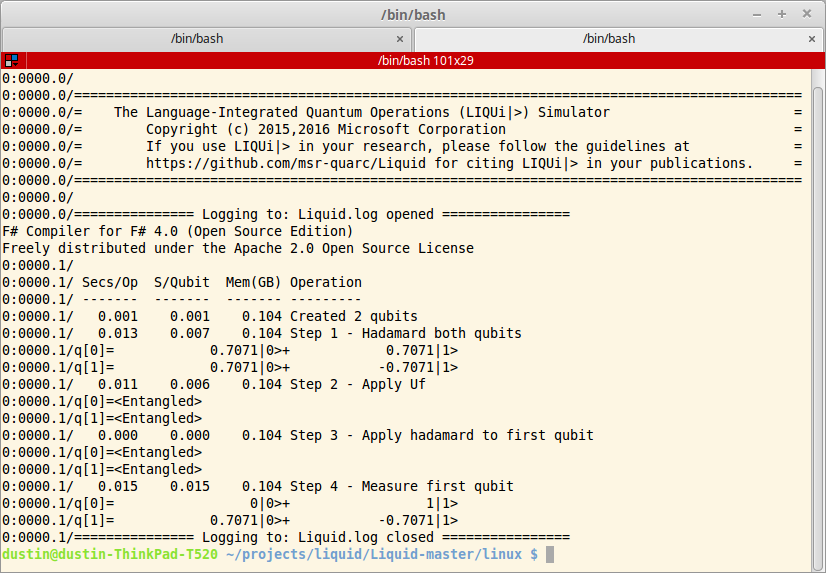
\includegraphics[scale=.45]{deutsch_screen} \\

Liquid supports printing and logging information as scripts are run. In our Deutsch's example we output the state vector
for each qubit after each gate is applied. The state vectors are output in bra-ket notation, unless the state is entangled,
in which case the string "entangled" is displayed. \\

Looking at the first qubit, at the end of the script, the state $\ket{0}$ has amplitude $0$,
and the state $\ket{1}$ has amplitude $1$, as expected for a balanced function.
\pagebreak

\section{Quantum Programming Language Theory}



$$$$
{\huge Preface and Overview of classical lambda calculi:}
$$$$


In the classical setting, various lambda calculi exist with different type systems.

These can be divided into the untyped lambda calculus, and a large number of important typed lambda calculi.

$$$$
{
\large Untyped lambda calculus:}
$$$$

The untyped lambda calculus is Turing complete: we can provide encodings of objects we care about in the form of terms in the untyped lambda calculus,
and the computational power of the untyped lambda calculus allows us to map inputs to outputs in terms of these encodings in arbitrary computable ways.

The problem with using untyped lambda calculi for computation lies in the great number of terms for which we cannot attach computational meaning, as well as the difficulty in reasoning about the behavior of programs, such as determining if they output a value of the form we are interested in.

$$$$
{
\large Typed lambda calculi:}
$$$$

Typed lambda calculi, the basis for typed programming languages, address this by providing a mechanism for rejecting certain programs which have undesirable properties, the most common of which being terminating computation in a term which does not correspond to a valid output of the program.

Type systems in general can do even more, and can verify more or less arbitrary properties of programs.

This is useful for the purpose of verifying the correctness of code, and for generation of code from a specification.
This is closely tied to applications in universal artificial intelligence and other important fields.

We are, however, limited by Rice's Theorem, so type systems cannot decidably differentiate arbitrary properties with certainty.

The type systems in the classical case therefore typically tackle this problem from two directions.

Either they start with a total language, which has only terminating programs, and then add functionality to increase the amount of computable functions in the language, or they start with a Turing complete language, and then add limitations on programs to reject more and more invalid programs.

In extreme cases, languages push the limits on Rice's theorem by allowing the programmer to assist the compiler in type checking programs by providing proofs that they are of the correct type.

$$$$
{
\Huge Quantum lambda calculi:}
$$$$


We are interested in how this pictures relates to the quantum case.
Before attempting to study quantum lambda calculi, however, we need to have a model of the untyped quantum lambda calculus.

$$$$
{
\large An Untyped Quantum lambda Calculus:}
$$$$

This is the main theoretical work for this report.
We focused on the paper "A Lambda Calculus for Quantum Computation" for this,
It is possible that there are other ways of creating an untyped quantum lambda calculus.
We found this presentation to be rather elegant.
When creating the quantum untyped lambda calculus from the previous section, we must satisfy many properties, including: 
$$$$
Our quantum untyped lambda calculus:
$$$$
1) should be Turing complete.$$$$
2) should resemble as closely as possible the classical untyped lambda calculus.$$$$
3) should have a universal set of quantum primitives in order to perform optimal quantum computation$$$$
4) should maintain invertibility of quantum computation.$$$$
5) should not terminate in a superposition that isn't properly normalized$$$$
$$$$

There are a few more technical properties as well that we might care about.


Since we start with the classical untyped lambda calculus, property 1 is satisfied, and while 2 is subjective it appears to be reasonably satisfied as well. One complaint is that our calculus works by recording histories, which may be too wasteful of space.
To achieve (3), we add any universal set of quantum primitives. For instance, the paper we examine suggests Rotation by $\pi/8$, H, and CNot.

To achieve (4), we record histories of our computation. That is, every small-step in our computation consists in
transforming lambda expression "h1; h2; ... hn; x" to "h1; h2; ... hn; x ; y" where y is the term we would obtain under standard reduction of x.
In other words, in addition to normalizing terms as we typically do in lambda calculus, we generate product states that repeatedly append lambda terms to represent the entire history of computation.
$$$$
While we will later modify this definition slightly, for now, our plan is for $\ket{H 0}$ to become $1/\sqrt{2} (\ket{H 0; 0} + \ket{H 0; 1})$
$$$$

Note that we now have invertibility, but adding histories causes problems with cancellation of terms with different histories.

In particular, computing  $\ket{H (H 0)}$ does not result in $\ket{0}$ in the computational register. The issue when computing this value, is that we cannot cancel a term with H 1 in its history with one that has H 0 in the same position in its history:
 $\ket{H (H 0)}$ normalizes to $\dfrac{1}{2} \ket{H (H 0)} \bigotimes (\ket{H 0; 0} + \ket{H 0; 1} + \ket{H 1; 0} - \ket{H 1; 1})$

 To fix this problem, a rather deep result is that the super position doesn't affect the structure of the computation: If we replace all 0 and 1 kets in the history with underscores, everything factors nicely, and $\ket{H (H 0)}$ evaluates to 0. The amazing thing about this is that everything is still invertible!
$$$$
$$$$
{
\Large Linearity:}
$$$$
$$$$

Other than the potential inefficiency associated with copying histories, there is only one problem remaining with the above presentation.
Any function that discards its argument loses information, and a function whose argument appears twice or more in its body can perform cloning.
$$$$
We need a mechanism for specifying which terms are linear, meaning they must be used exactly once, and which are non-linear, or classical, meaning they can be copied or discarded at will. We allow for terms to be linear or non-linear, and we allow for the argument to lambda abstractions to be linear or non-linear. What remains is a lot of technical details to show that linear terms aren't promoted to non-linear terms when they should not be, etc.
$$$$
We can think of linear terms as representing arbitrary quantum computation, while non-linear terms represent classical computation.
One interesting question is whether this can be formulated in a non-conservative manner. That is, a calculus that allows linear terms to be promoted to non-linear terms exactly when they are classical. 
$$$$

$$$$
$$$$
{
\Large Plan for the final:}
$$$$
$$$$

We have seen how the untyped classical lambda calculus can be translated into an untyped quantum lambda calculus.
This is however, an extremely small result. What is really interesting is not that quantum computation can be formulated in terms of lambda calculi,
but that we can create type systems for quantum lambda calculi.

This is what will allow us ultimately (though far outside the scope of this project) to verify properties of quantum programs, and to search the space of quantum programs.

We in particular are interested in the relationship between classical linearity and quantum computation.

$$$$
Curry Howard Correspondence
$$$$
The curry howard correspondence is a relationship between logic and typed lambda calculi.
In particular therefore, we are interested in quantum logic.
Quantum logic is related to linear logic, so linear logic may come up in the final presentation due to its indirect connection to quantum type systems.




\end{document}